\documentclass{article}


\usepackage{style}

\usepackage[utf8]{inputenc}
\usepackage[T1]{fontenc}
\usepackage{hyperref}
\usepackage{url}
\usepackage{booktabs}
\usepackage{amsfonts}
\usepackage{nicefrac}
\usepackage{microtype}
\usepackage{graphicx}
\graphicspath{{media/}}

%% Title
\title{Veevo Health: Heart Age Calculator}

\author{Arvind Srivastav \\
Veevo Health, San Francisco, CA, USA \\
\texttt{arvind@veevo.health}}

\begin{document}
\maketitle

\begin{abstract}
Heart age reframes multi-factorial cardiovascular risk into an intuitive metric that facilitates communication and motivates prevention. We present the design and validation of the Veevo Health Heart Age Calculator, which couples contemporary risk equations with a US-representative, age- and sex-specific healthy comparator derived from NHANES 2015--2023. We emphasize methodological transparency sufficient for scientific appraisal while limiting disclosure of proprietary implementation details. Using survey-weighted models and a principled healthy comparator (non-smoker; diabetes-free; not on lipid- or blood-pressure-lowering therapy; desirable lipids; physiologic age-trending systolic blood pressure), we quantify population heart-age discordance and demonstrate face-valid patterns across age and sex.
\end{abstract}

% keywords can be removed
\keywords{heart age \and cardiovascular risk \and PREVENT \and NHANES \and healthy comparator \and prevention}

\section{Background and Rationale}
Absolute cardiovascular risk scores---while foundational for clinical decision-making---can be abstract and difficult to communicate. Heart age instead asks: \emph{at what chronological age would an average healthy peer have the same predicted risk as this individual?} Prior work has demonstrated that such age-based framing improves patient understanding and willingness to act on prevention~\cite{Blaha2021JAHA}.

Veevo's approach aligns with this communication objective while adhering to modern risk prediction and population-representative comparators. At a high level, our system (i) estimates an individual's 10-year atherosclerotic cardiovascular disease (ASCVD) risk using contemporary, sex-specific equations; (ii) defines a healthy age- and sex-specific comparator profile; and (iii) solves for the reference age at which comparator risk equals the individual's risk. We report the resulting \emph{heart age} and its difference from chronological age (\emph{discordance}).

\section{Healthy Comparator (Reference) Profile}
We follow the abstract comparator design used in prior work~\cite{Blaha2021JAHA}: the comparator is non-diabetic, a non-smoker, not receiving lipid- or blood-pressure-lowering therapy, and has desirable renal function. To avoid disclosing implementation specifics, we summarize the salient anchors that define our comparator:
\begin{itemize}
  \item HDL-C fixed at 55 mg/dL for women and 45 mg/dL for men (consistent with cardiometabolic literature and patient-facing guidance).
  \item Non-HDL-C fixed at 120 mg/dL, a stringent but attainable non-HDL target reflective of contemporary prevention goals.
  \item eGFR set to 90 mL/min/1.73m$^2$ (physiologically normal renal function).
  \item Systolic blood pressure (SBP) is \textbf{not fixed}. Because SBP rises with age even among healthy individuals, we estimate \textbf{age- and sex-specific healthy SBP} from NHANES using survey-weighted regression restricted to a low-risk subpopulation (details below). For women, we allow a linear spline at the typical menopause age of 52 years to capture the known inflection in lipid and hemodynamic physiology~\cite{ClevelandClinicMenopause}.
\end{itemize}

\subsection{NHANES-Derived Healthy SBP}
To emulate a ``generally healthy'' reference, we begin with NHANES 2015--2023 participants and restrict to individuals who are: non-smokers; free of diabetes; BMI $<$ 30 kg/m$^2$; SBP $<$ 140 mmHg; and not on antihypertensive therapy. We then fit sex-specific, survey-weighted linear models of SBP on age (men: linear; women: linear with a 52-year knot to reflect menopause physiology~\cite{ClevelandClinicMenopause}). Predicted values from these models define the comparator SBP across ages. Figure~\ref{fig:healthy-sbp} illustrates the resulting curves.

\begin{figure}
  \centering
  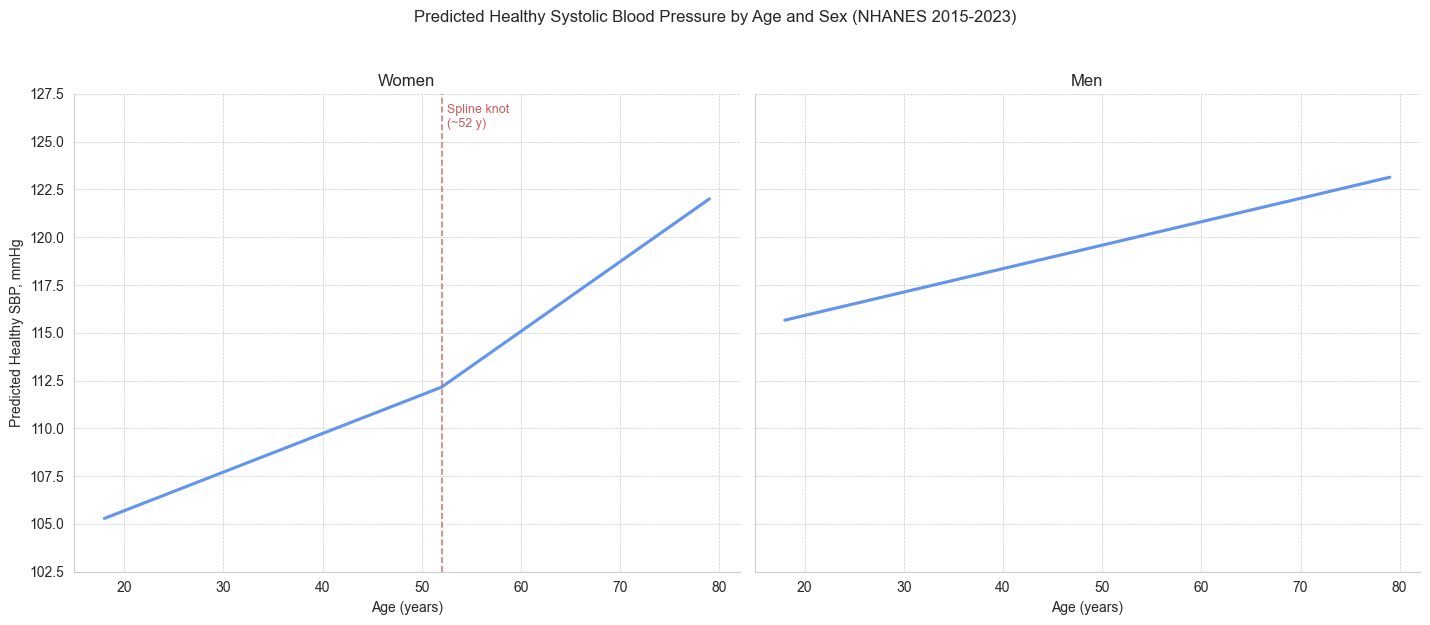
\includegraphics[width=0.95\textwidth]{healthy_sbp_by_age.png}
  \caption{Predicted healthy SBP by age and sex (NHANES 2015--2023, survey-weighted). Women include a linear spline with a 52-year knot to accommodate post-menopausal physiology.}
  \label{fig:healthy-sbp}
\end{figure}

\section{Risk Model and Heart-Age Mapping}
We operationalize heart age by equating an individual's absolute risk to the comparator's absolute risk at an unknown age and solving for that age. We employ contemporary, parallel sex-specific equations over a 10-year horizon (ASCVD outcome) with predictors age, SBP (with treatment indicator), smoking, diabetes, non-HDL-C, HDL-C, eGFR, antihypertensive therapy, and statin therapy. Interaction and transformation structure follow the published framework. Exact coefficients and solver details are proprietary; however, our implementation conforms to the published variable set and functional motifs used by modern equations.

\section{Data Source and Analytic Principles}
\textbf{Data.} U.S. National Health and Nutrition Examination Survey (NHANES) 2015--2023 cycles were used to estimate comparator parameters and to describe national patterns of heart-age discordance. We combined cycles under the complex survey design and used MEC examination weights to recover population-representative estimates.

\textbf{Survey weighting.} All descriptive estimates and regression models were \emph{survey-weighted} using NHANES examination weights so that the results reflect the U.S. civilian, non-institutionalized population rather than the raw sample.

\textbf{Low-risk comparator subset.} For comparator SBP modeling, we restricted to adults 18--79 years who are non-smokers, diabetes-free, BMI $<$ 30 kg/m$^2$, SBP $<$ 140 mmHg, and not on blood-pressure medication. Lipid anchors (HDL-C, non-HDL-C) were set to desirable constants as noted above.

\section{Population Heart-Age Discordance (NHANES 2015--2023)}
We applied the heart-age mapping to NHANES adults 30--79 years to quantify discordance (heart age minus chronological age). Discordance was categorized as: $>$10 years older; 5--10 years older; within 5 years; and $>$5 years younger. Figure~\ref{fig:discordance} shows the sex-stratified, age-banded, \emph{survey-weighted} population counts in millions.

\begin{figure}
  \centering
  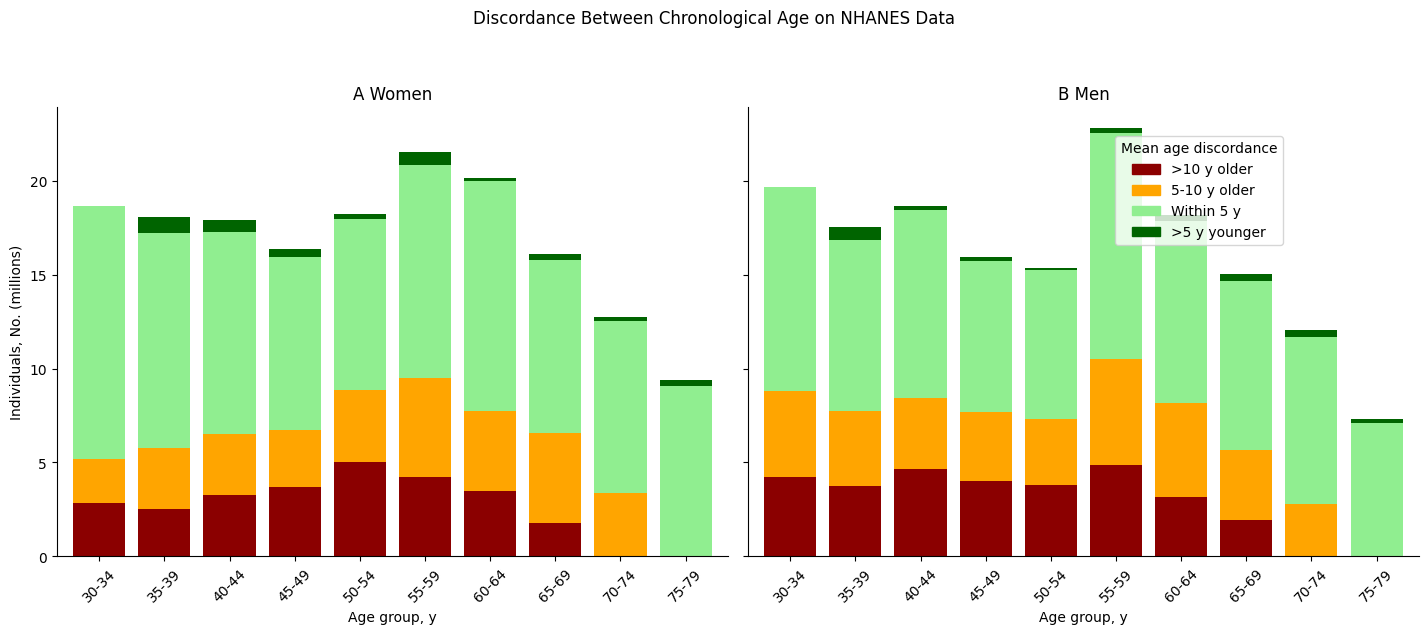
\includegraphics[width=0.95\textwidth]{heart_age_discordance.png}
  \caption{Discordance between heart age and chronological age by age-band and sex (NHANES 2015--2023). Bars sum to estimated U.S. population counts (millions) within each stratum.}
  \label{fig:discordance}
\end{figure}

\subsection{Distribution Across Discordance Buckets}
For clinical interpretability, we summarize the fraction of adults within each discordance category across 5-year age bands and by sex. Table~\ref{tab:discordance-fractions} provides the structure; values are computed directly from the survey-weighted aggregation and are available in the project artifacts.

% Table inlined (four buckets incl. >5 younger)
\begin{table}
  \centering
  \caption{Fraction of U.S. adults (survey-weighted) by heart-age discordance category, age-band, and sex (NHANES 2015--2023).}
  \label{tab:discordance-fractions}
  \begin{tabular}{lcccccccc}
    \toprule
    & \multicolumn{4}{c}{Women} & \multicolumn{4}{c}{Men} \\
    \cmidrule(r){2-5} \cmidrule(r){6-9}
    Age band & $>10$ older & 5--10 older & Within 5 & $>5$ younger & $>10$ older & 5--10 older & Within 5 & $>5$ younger \\
    \midrule
    30--34 & 15.2 & 12.6 & 72.3 & 0.0 & 21.6 & 23.3 & 55.1 & 0.0 \\
    35--39 & 13.8 & 18.0 & 63.4 & 4.9 & 21.4 & 22.7 & 52.2 & 3.8 \\
    40--44 & 18.1 & 18.2 & 59.9 & 3.7 & 24.9 & 20.5 & 53.6 & 1.0 \\
    45--49 & 22.6 & 18.6 & 56.2 & 2.6 & 25.3 & 23.1 & 50.2 & 1.4 \\
    50--54 & 27.6 & 21.1 & 49.7 & 1.6 & 24.7 & 22.8 & 51.6 & 0.9 \\
    55--59 & 19.7 & 24.4 & 52.8 & 3.1 & 21.4 & 24.8 & 52.9 & 1.0 \\
    60--64 & 17.2 & 21.3 & 60.7 & 0.9 & 17.3 & 27.6 & 53.6 & 1.5 \\
    65--69 & 11.1 & 29.7 & 57.4 & 1.8 & 12.8 & 25.0 & 59.7 & 2.5 \\
    70--74 & 0.0 & 26.4 & 71.7 & 1.9 & 0.0 & 23.1 & 73.7 & 3.1 \\
    75--79 & 0.0 & 0.0 & 96.6 & 3.4 & 0.0 & 0.0 & 97.2 & 2.8 \\
    \bottomrule
  \end{tabular}
\end{table}

\section{Interpretation}
Three robust patterns emerge:
\begin{enumerate}
  \item \textbf{Age gradient.} The share of individuals with heart age $>$ chronological age increases with age, particularly in men, consistent with accumulation of risk factors.
  \item \textbf{Sex differences.} Women display lower discordance at younger ages, with a convergence around the mid- to late-50s consistent with post-menopausal physiology~\cite{ClevelandClinicMenopause}.
  \item \textbf{Comparator face validity.} Using age-trending, healthy SBP (rather than a fixed 110 mmHg) avoids overstating youthfulness in older adults and reflects physiologic realities.
\end{enumerate}

\section{Implementation Notes and Guardrails}
\begin{itemize}
  \item The heart-age solver safeguards against extrapolation by constraining the solution to validated age bounds (30--79 years).
  \item Inputs are validated for physiologic plausibility and missingness; default imputation for non-critical inputs adheres to conservative, health-preserving values.
  \item Outputs display heart age and discordance with context-sensitive messaging to promote guideline-concordant prevention rather than risk minimization alone.
\end{itemize}

\section{Limitations}
Our white paper intentionally withholds certain implementation specifics to preserve product differentiation. Nonetheless, all choices (predictor set, variable transformations, and comparator anchors) are consistent with peer-reviewed paradigms. As with all survey-based generalizations, residual confounding and measurement error are possible despite weighting and restriction.

\section{Conclusion}
Veevo's Heart Age Calculator translates complex risk into a single, understandable number that encourages preventive action. By pairing contemporary risk equations with a physiologically grounded, NHANES-derived healthy comparator---and by reporting population-discordance patterns in U.S.-representative data---we demonstrate both rigor and relevance while maintaining proprietary protections.

\section*{Acknowledgments}
We thank the participants and staff of NHANES and the cardiovascular prevention community for foundational advances in risk modeling and communication.

%Bibliography (inline minimal entries)
\begin{thebibliography}{9}
\bibitem[Blaha(2021)]{Blaha2021JAHA} Blaha, M.J.; Naazie, I.N.; Cainzos-Achirica, M.; et al. Derivation of a Coronary Age Calculator Using Traditional Risk Factors and Coronary Artery Calcium: The Multi-Ethnic Study of Atherosclerosis. \emph{J Am Heart Assoc}. 2021;10(6):e019351. doi:10.1161/JAHA.120.019351. Available at: \url{https://pubmed.ncbi.nlm.nih.gov/33663219/}.
\bibitem[Cleveland Clinic(2024)]{ClevelandClinicMenopause} Cleveland Clinic. Menopause. 2024. Available at: \url{https://my.clevelandclinic.org/health/diseases/21841-menopause}. Accessed 2025-10-24.
\end{thebibliography}

\end{document}
